\chapter{Analysis}

Tree building was done on an HP Z820 Workstation with an Intel Xeon E5-2650,
256GiB RAM, and a 1TB and 2TB Samsung 850 Pro SSD’s. The MapDB library was used
for point storage by tree cell and index and in place of in-memory storage, a
file system map was used and stored on the 1TB SSD. The input point data was
stored on the 2TB SSD and the output tree structure was written there as well;
this was to make sure the MapDB file was not interfering with reading or writing
the point data.

The data set used was a subset of the Morro Bay area from the San Simeon, CA
dataset \cite{15_opentopo_morrobay}. The area used falls within (-120.88, 35.36)
and (-120.84, 35.40).
It contains a total of 163,251,931 points.

\section{Octree and Icosatree Building Stastics}

The Octree building statistics were run with a few different sub-cell sizes. A
Table of sub-cell size, elapsed times, max and average points per cell, max tree
depth, directory and file count, and total file size can be found in Tables
\ref{table:octreeStats} and \ref{table:icosatreeStats}. With the Icosatree,
attempts were made initially using barycentric coordinates as the basis of the
indexing system but because barycentric coordinates are a weighted average
position within the triangle and not an absolute weight for each vertex the
system didn’t work as intended. Later, a naive axis-aligned index was used in
the same fashion as the Octree sub-cell index but most of the index range went
unused. Finally, a triangular coordinate system was developed that computes a
position based on the projected position along two of the triangular edges. The
triangular coordinate system computes a sub-cell index by splitting one edge
into n-sections. Then, a second edge is also split into n-sections, however, it
is numbered in both directions; this creates two columns of sub-cells oriented
left-to-right and right-to-left. Then, each sub-cell is numbered with a triple
coordinate index. A point is inserted into a sub-cell along the top face of the
triangular prism volume and then offset by depth into the volume by splitting
the depth by m-sections. A diagram of the triangular coordinates can be seen in
Figure \ref{fig:triCoords}.

\begin{figure}[htp]
\begin{center}
  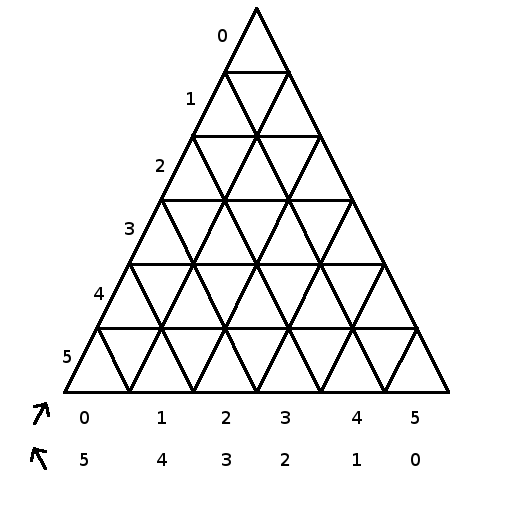
\includegraphics[width=3.0in]{images/triangularCoordinates.png}
  \caption{Triangular Coordinates}
  \label{fig:triCoords}
\end{center}
\end{figure}

\begin{table}[htp]
\caption{Octree Building Statistics}
\resizebox{\textwidth}{!}{%
  \begin{tabular}{lllcccclll}
    \toprule
    \shortstack{Sub-Cell\\Size} & \shortstack{Tree\\Creation\\Time} & \shortstack{Cells\\Created} & \shortstack{Filesystem\\Export Time} & \shortstack{Max Points\\Per Cell} & \shortstack{Average Points\\Per Cell} & \shortstack{Max\\Tree Depth} & \shortstack{Directory\\Count} & \shortstack{File\\Count} & \shortstack{Total\\File Size}\\
    \midrule
      50x50x50 & 5h 8m & 1,093,494 & 20m 48s & 15548 & 150 & 32 & 1,093,494 & 2,186,989 & 11 GiB, 124 MiB \\
      100x100x100 & 4h 42m & 389,771 & 15m 55s & 44223 & 419 & 31 & 389,771 & 779,543 & 11 GiB, 109 MiB \\
    \bottomrule 
  \end{tabular}}
\label{table:octreeStats}
\end{table}

\begin{table}[htp]
\caption{Icosatree Building Statistics}
\resizebox{\textwidth}{!}{%
  \begin{tabular}{lllcccclll}
    \toprule
    \shortstack{Sub-Cell\\Size} & \shortstack{Tree\\Creation\\Time} & \shortstack{Cells\\Created} & \shortstack{Filesystem\\Export Time} & \shortstack{Max Points\\Per Cell} & \shortstack{Average Points\\Per Cell} & \shortstack{Max\\Tree Depth} & \shortstack{Directory\\Count} & \shortstack{File\\Count} & \shortstack{Total\\File Size}\\
    \midrule
      100x100x100 & 5h 25m & 725,672 & 26m 41s & 17123 & 225 & 32 & 725,672 & 1,451,345 & 11 GiB, 115 MiB \\
      100x20 & 7h 18m & 653,475 & 32m 38s & 10233 & 250 & 31 & 653,475 & 1,306,951 & 11 GIB, 114 MiB \\
      100x100 & 6h 27m & 583,163 & 25m 43s & 14569 & 280 & 31 & 583,163 & 1,166,327 & 11 GiB, 112 MiB \\
      150x100 & 6h 14m & 340,758 & 23m 54s & 22618 & 480 & 30 & 340,758 & 681,517 & 11 GiB, 107 MiB \\
      200x100 & 5h 49m & 235,156 & 20m 4s & 38081 & 695 & 29 & 235,156 & 470,313 & 11 GiB, 105 MiB \\
    \bottomrule 
  \end{tabular}}
\label{table:icosatreeStats}
\end{table}

Originally, a barycentric coordinate was used for inserting points into Icosatet
sub-cells. However, once the system was tested it showed that because the
barycentric coordinates cannot be positioned along two axes as with the
Cartesian coordinate based Octree, all of the points were skewed towards one
corner of the Icosatet. As a temporary replacement, the Octree split algorithm
was used but caused a large number of sub-cells to be outside the bounds of the
Icosatet and effectively wasted. Eventually, the triangular coordinate system
was developed which alleviated the drawbacks of the other algorithms tested and
fit well with the use case.

\section{Point Selection and Triangulation}

The Point Selection and Triangulation is implemented with a number of options.
First, the CAST algorithm used a Marching Cubes algorithm to compute point
densities and prune all points above a certain threshold; this was implemented
early on but the issues with using a structured point cloud like San Simeon, CA
became apparent. The marching cubes approach ended up removing most of the
points selected or almost none at all. In the end, the screen-space lasso was
the only portion of the paper implemented. This created a projected frustum into
the scene which was used to cull points outside of the selection.

Next, the screen-space point pruning was implement in a few different ways. The
application of which is tunable as well as the run order of each portion
implemented. The first pruning algorithm added was a naive altitude offset where
the min/max altitude range of all points selected was computed and then the nth
lowest percentage were removed. Second, an orthonormal threshold was added
where, for each point, the k-nearest neighbors were queried. The orthonormal
vector was found by computing the eigenvectors for the set of neighbors and if
this vector was within a certain threshold of the global eigenvector normal, the
point was discarded. Last, the screen-space operator pruning algorithm was used
to remove any points that were obstructed by other points by using distance to
the camera and an angle threshold between the vector from the tested point and
all other points in the selection. If the tested point was behind another point
and the angle between its camera vector and the other points’ camera vector
failed a threshold value, the point was discarded.

Once the point pruning is completed, all points are converted into x,y global
eigenvector space and inserted into a map to preserve the local-to-world
position pair. The local-space vertices were then sent through a Delaunay
triangulation algorithm pass and all triangles exported are then converted back
into world coordinates using the local-to-world coordinate mappings.

A few point selection and triangulation examples can be found in Figures
\ref{fig:pointSelection2}, \ref{fig:triangulation2}, \ref{fig:triangulation3},
and \ref{fig:triangulation4}.

\begin{figure}[htp]
\begin{center}
  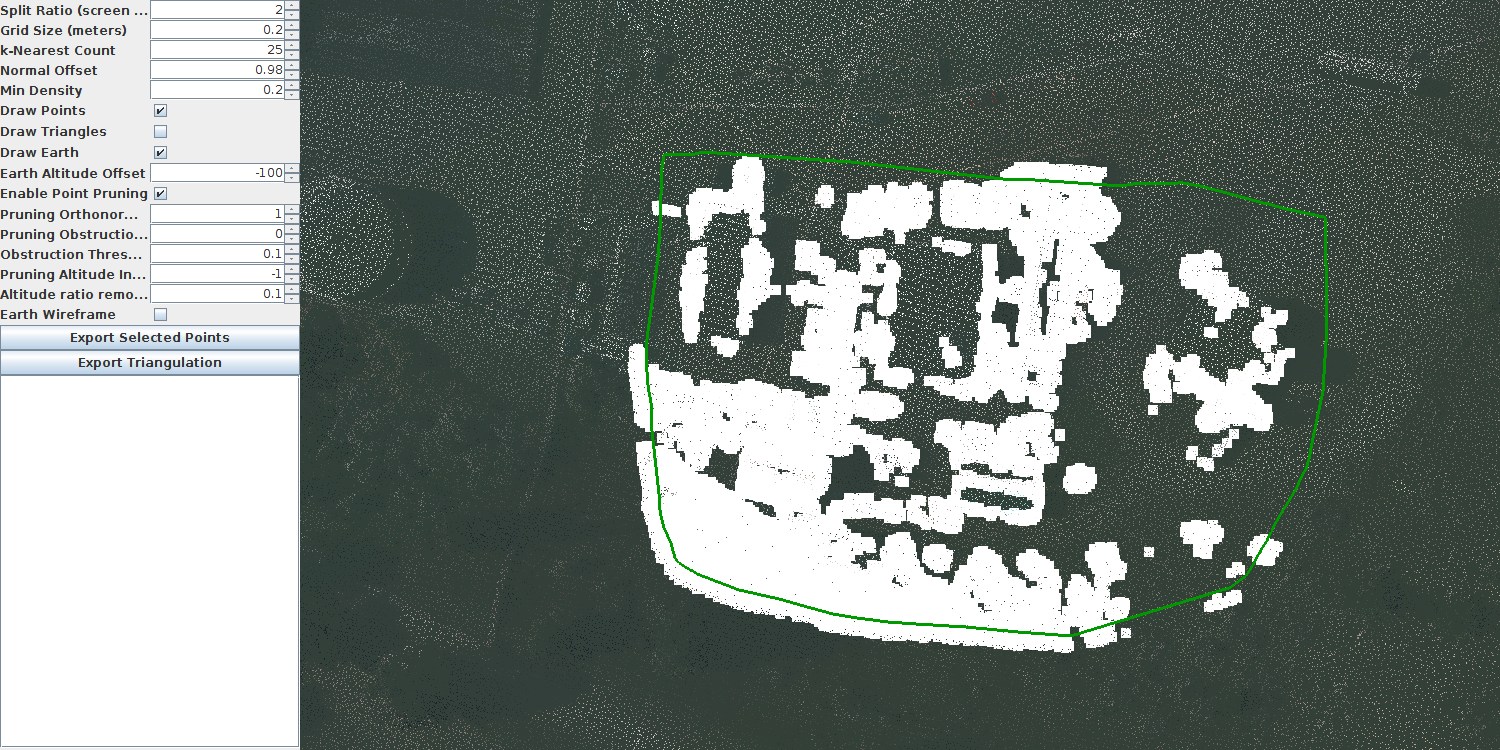
\includegraphics[width=6.0in]{images/pointSelection2.png}
  \caption{Point Selection with Lasso}
  \label{fig:pointSelection2}
\end{center}
\end{figure}

\begin{figure}[htp]
\begin{center}
  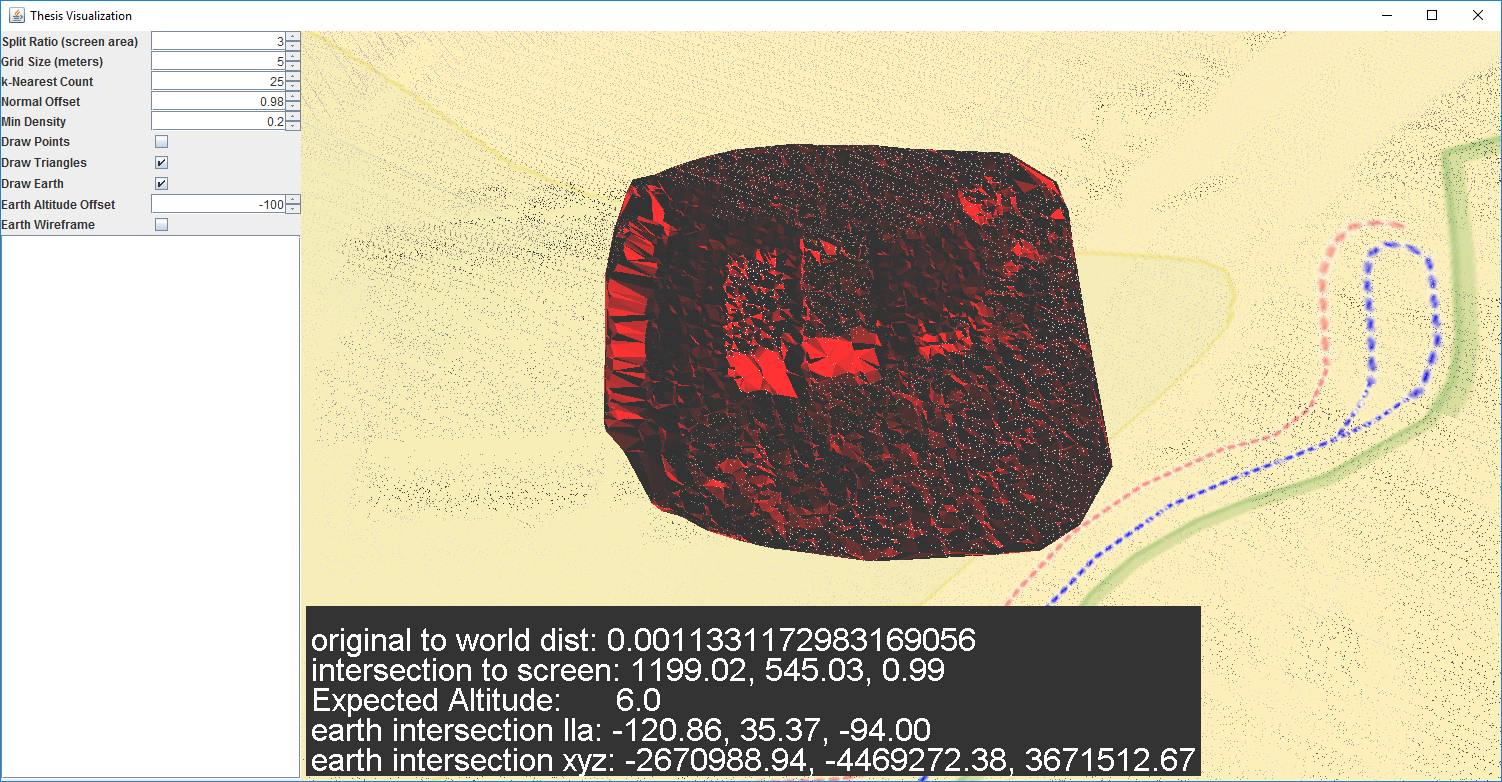
\includegraphics[width=6.0in]{images/triangulation2.png}
  \caption{Selection Triangulation}
  \label{fig:triangulation2}
\end{center}
\end{figure}

\begin{figure}[htp]
\begin{center}
  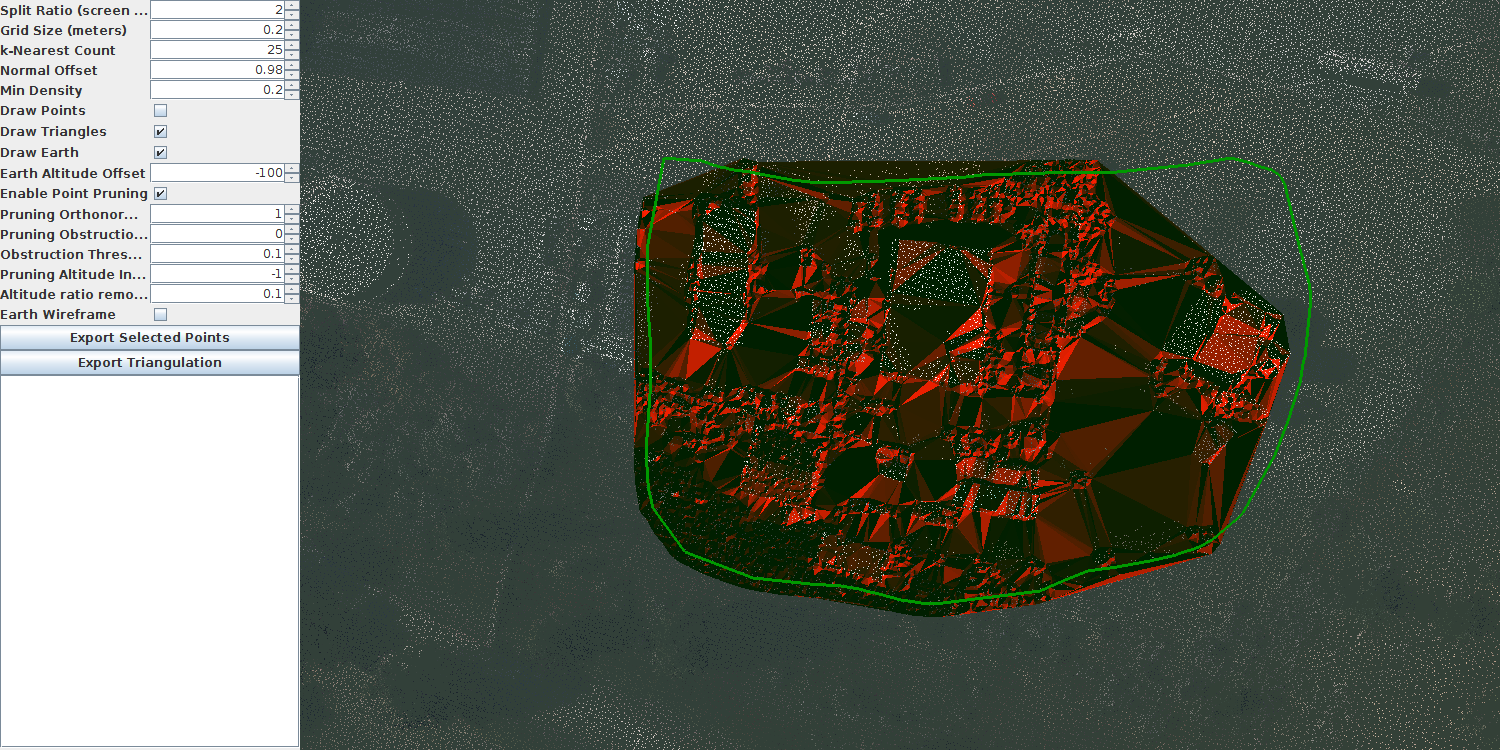
\includegraphics[width=6.0in]{images/triangulation3.png}
  \caption{Selection Triangulation with Obstruction Pruning}
  \label{fig:triangulation3}
\end{center}
\end{figure}

\begin{figure}[htp]
\begin{center}
  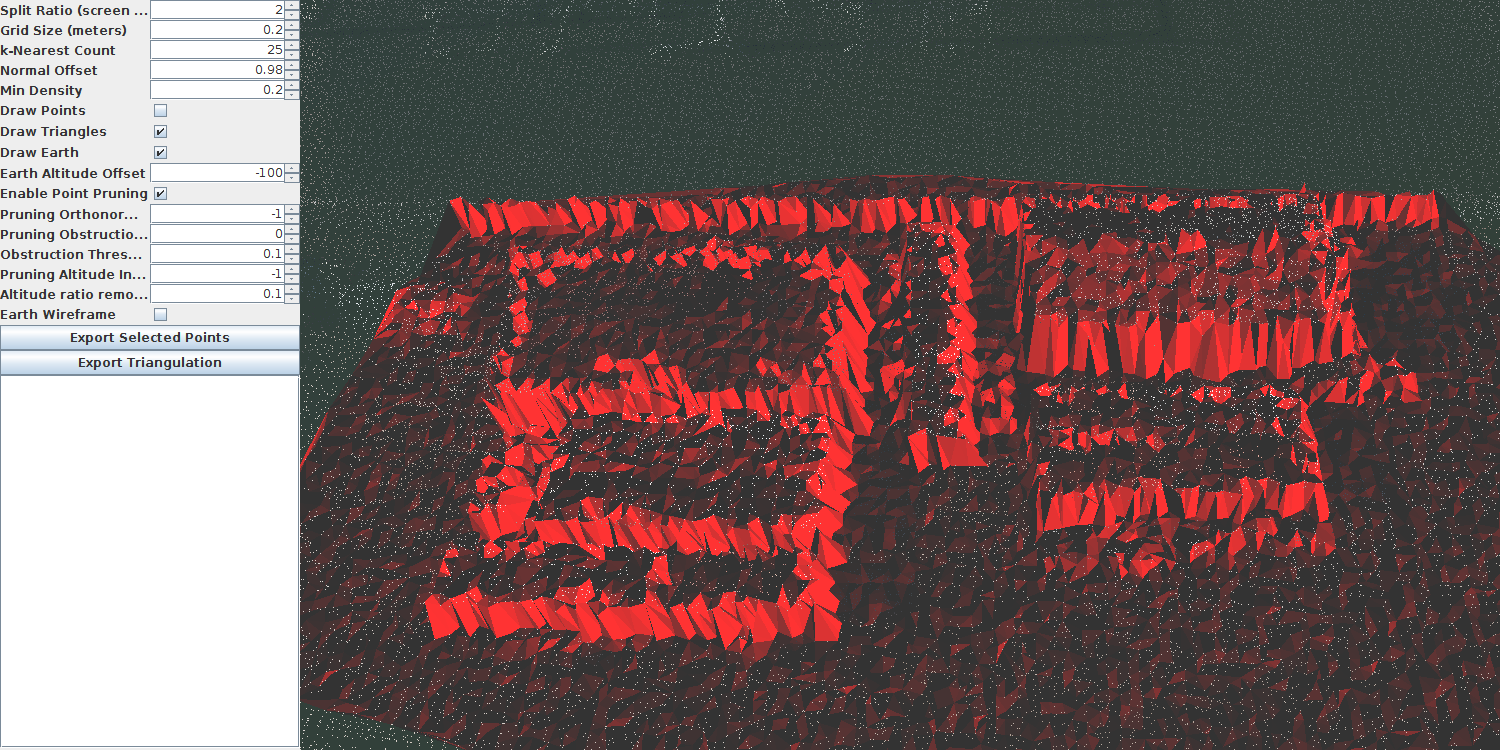
\includegraphics[width=6.0in]{images/triangulation4.png}
  \caption{Selection Triangulation Closeup}
  \label{fig:triangulation4}
\end{center}
\end{figure}

\section{Octree vs Icosatree Cell Size and Rendering Statistics}

The Octree was initially chosen as the data structure for the point cloud data
as it allowed a global dataset to be handled without the need to deal with
geodetic coordinates and that the Cartesian coordinate space parallels directly
with the graphics pipeline. The axis-aligned nature of the cells also allows for
efficient culling of the dataset during rendering. However, the Octree structure
does not follow the projected surface of the Earth well and there is a large
portion of the Octree structure that is never used. The Icosatree structure was
chosen as a potential alternative because it aligns with the Earth’s projected
surface more closely, each cell in the tree splits into child cells whose volume
can be filled more efficiently, and the handling of the tree file structure is
identical to the Octree version so can be used as a direct replacement with very
little additional modification and the tree can be traversed with little
additional overhead. Also, because the tree cells are filled more efficiently,
data usage in the vertex buffer should be less wasteful compared with the Octree
implementation. Below, in \ref{table:octreeCellStats} and
\ref{table:icosatreeCellStats}, are tables of sub-cell sizes, including
Cartesian dimensions, surface area, and volume for cells at a number of select
tree depths.

\begin{table}[htp]
\caption{Octree Cell Statistics}
\resizebox{\textwidth}{!}{%
  \begin{tabular}{lllllll}
    \toprule
      Tree Depth & Type & X-Span (m) & Y-Span (m) & Z-Span (m) & Side Area ($m^2$) & Volume ($m^3$) \\
    \midrule
      18 & AABB & 64 & 64 & 64 & 4096 & 262144 \\
      19 & AABB & 32 & 32 & 32 & 1024 & 32768 \\
      20 & AABB & 16 & 16 & 16 & 256 & 4096 \\
      21 & AABB & 8 & 8 & 8 & 64 & 512 \\
      22 & AABB & 4 & 4 & 4 & 16 & 64 \\
    \bottomrule 
  \end{tabular}}
\label{table:octreeCellStats}
\end{table}

\begin{table}[htp]
\caption{Icosatree Cell Statistics}
\resizebox{\textwidth}{!}{%
  \begin{tabular}{lllllllll}
    \toprule
      Tree Depth & Type & X-Span (m) & Y-Span (m) & Z-Span (m) & Depth (m) & Top Area ($m^2$) & Bottom Area ($m^2$) & Volume ($m^3$) \\
    \midrule
      18 & Triangle Prism & 83.7769 & 95.9998 & 64.0 & 29.8935 & 2709.8502 & 2709.8296 & 81006.642 \\
      19 & Triangle Prism & 41.8885 & 48.0 & 32.0 & 14.9468 & 677.4626 & 677.46 & 10125.8496 \\
      20 & Triangle Prism & 20.9443 & 24.0 & 16.0 & 7.4734 & 169.3656 & 169.3653 & 1265.7324 \\
      21 & Triangle Prism & 10.4721 & 12.0 & 8.0 & 3.7367 & 42.3414 & 42.3414 & 158.2166 \\
      22 & Triangle Prism & 5.2361 & 6.0 & 4.0 & 1.8683 & 10.5854 & 10.5853 & 19.7771 \\
    \bottomrule 
  \end{tabular}}
\label{table:icosatreeCellStats}
\end{table}

As can be seen from the tables above, The dimensions and volumes of the two tree
variations are comparable in absolute Cartesian bounds but their internal
volumes are much different. With the Icosatree cells being smaller but aligned
with the projected surface of the dataset they are filled more efficiently as
seen in Tables \ref{table:octreeStats} and \ref{table:icosatreeStats}. This
allows the rendering system to display fewer cells in order to render the same
amount of data while only adding a small amount of processing time when
computing frustum culling per cell which, overall, is still comparable by per
cell time (0.16 ms/cell vs. 0.19 ms/cell) as seen in Table
\ref{table:renderStats10}. However, it also adds a bit of point overdraw where
the cells that fill the frustum contain more points outside the viewable area
but are still drawn as their parent cell intersects the frustum and contains
some points within this area. Since the cell fits better with the dataset
projection, points will tend to fill the larger, less deep, cells in the tree.
The oriented axis cells perform better than the axis-aligned cells as seen by
comparing the Octree performance and the Icosatree with axis-aligned cells
compared to the Icosatree with oriented cells. The test performed below was on
the 100x100x100 sub-cell datasets with the level-of-detail set to maximum; this
requires a higher-than-normal per-frame time but was used to show the tree
rendering between each type as close to comparable as possible. The camera was
set at a specific location before starting the application so that each run was
consistent. An example of the rendering result can be seen in Figure
\ref{fig:rendering10}.

\begin{table}[htp]
\caption{Rendering Statistics (depth = 10.0)}
\resizebox{\textwidth}{!}{%
  \begin{tabular}{llllll}
    \toprule
      Cell Type & Point Count & Cell Count & Culling & Rendering & Building Bounds \\
    \midrule
      Icosatree (100x100) & 3355393 & 1276 & 252 ms & 1 ms 172 $\mu$s & 265 $\mu$s \\
      Icosatree (150x100) & 6065591 & 1533 & 236 ms & 1 ms 402 $\mu$s & 220 $\mu$s \\
      Icosatree (200x100) & 7325988 & 1522 & 187 ms & 1 ms 765 $\mu$s & 325 $\mu$s \\
      Octree (AABB) & 3692901 & 630 & 103 ms & 755 $\mu$s & 91 $\mu$s \\
    \bottomrule 
  \end{tabular}}
\label{table:renderStats10}
\end{table}

\begin{figure}[htp]
\begin{center}
  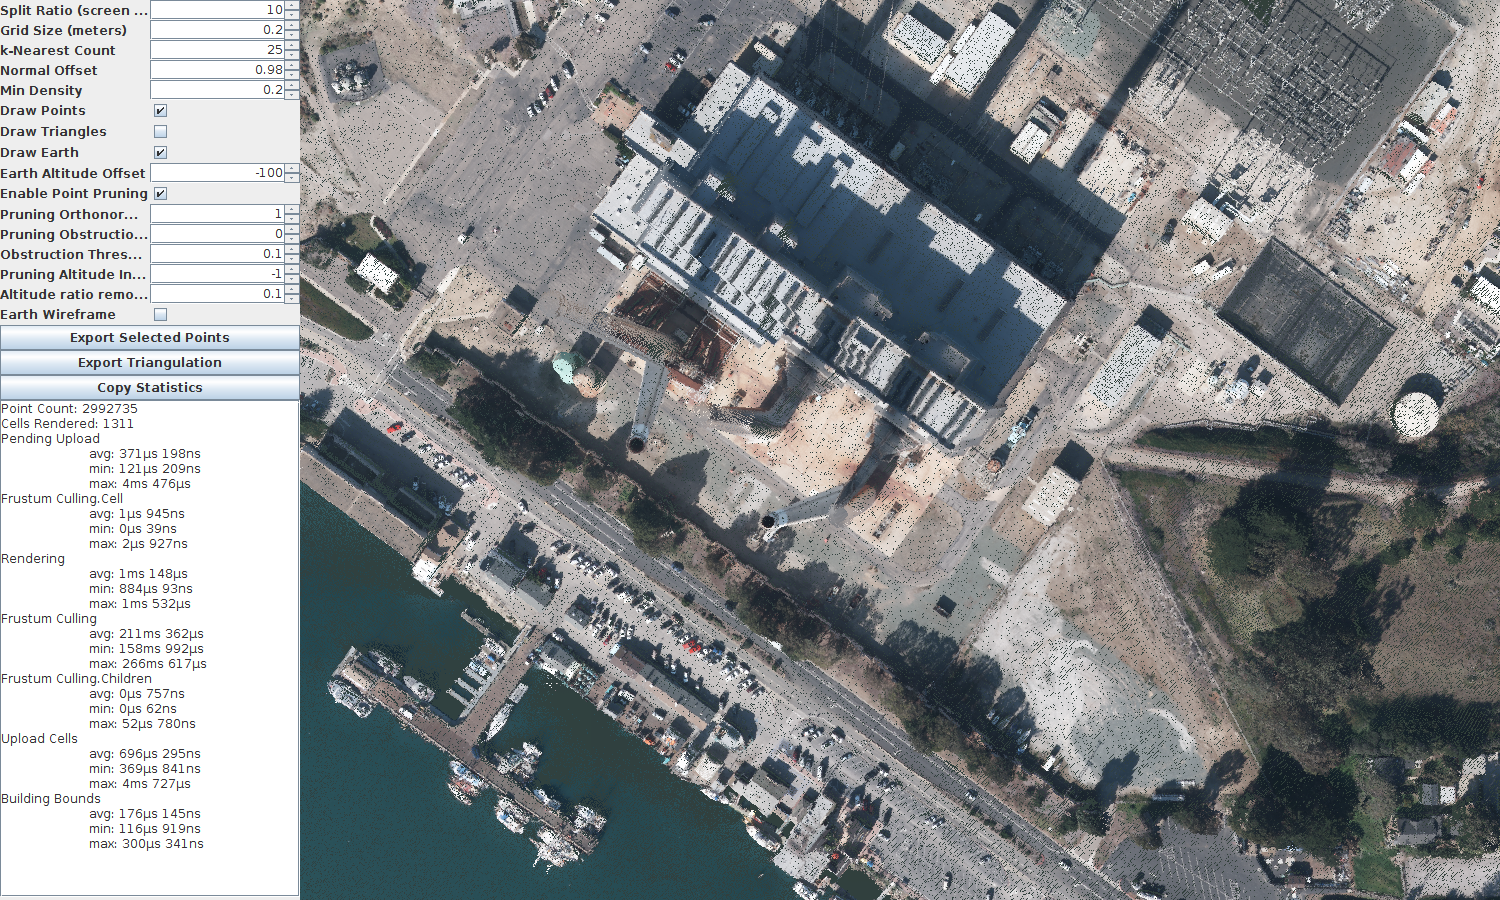
\includegraphics[width=6.0in]{images/rendering10.png}
  \caption{Rendering Statistics Sample Image (depth = 10.0)}
  \label{fig:rendering10}
\end{center}
\end{figure}

If the depth ratio is reduced to a more reasonable use-case, the comparisons
between using the Octree and Icosatree become less pronounced and more
manageable as seen in Tables \ref{table:renderStats3} and
\ref{table:renderStats6}.
The number of points rendered is slightly higher in the Icosatree implementation
than with the Octree, and per-frame times are increased as well. This is due in
part to the smaller altitude component of the icosahedron cell handling less
point data than the much more massive Octree cells. As seen in Tables
\ref{table:octreeCellStats} and \ref{table:icosatreeCellStats}, the depth of the
icosahedron cells limits the amount of data the cells can handle vertically
along the projected surface when compared to the Octree cells. In future
implementations, this might be alleviated by not splitting every cell along its
depth; such as all cells above a certain depth threshold or every third split,
for example.

\begin{table}[htp]
\caption{Rendering Statistics (depth = 3.0)}
\resizebox{\textwidth}{!}{%
  \begin{tabular}{llllll}
    \toprule
      Cell Type & Point Count & Cell Count & Culling & Rendering & Building Bounds \\
    \midrule
      Icosatree (100x100) & 1097116 & 200 & 67 ms & 636 $\mu$s & 53 $\mu$s \\
      Icosatree (150x100) & 2280826 & 201 & 47 ms & 408 $\mu$s & 60 $\mu$s \\
      Icosatree (200x100) & 3825534 & 201 & 96 ms & 332 $\mu$s & 52 $\mu$s \\
      Octree (AABB) & 880582 & 99 & 39 ms & 379 $\mu$s & 35 $\mu$s \\
    \bottomrule 
  \end{tabular}}
\label{table:renderStats3}
\end{table}

\begin{figure}[htp]
\begin{center}
  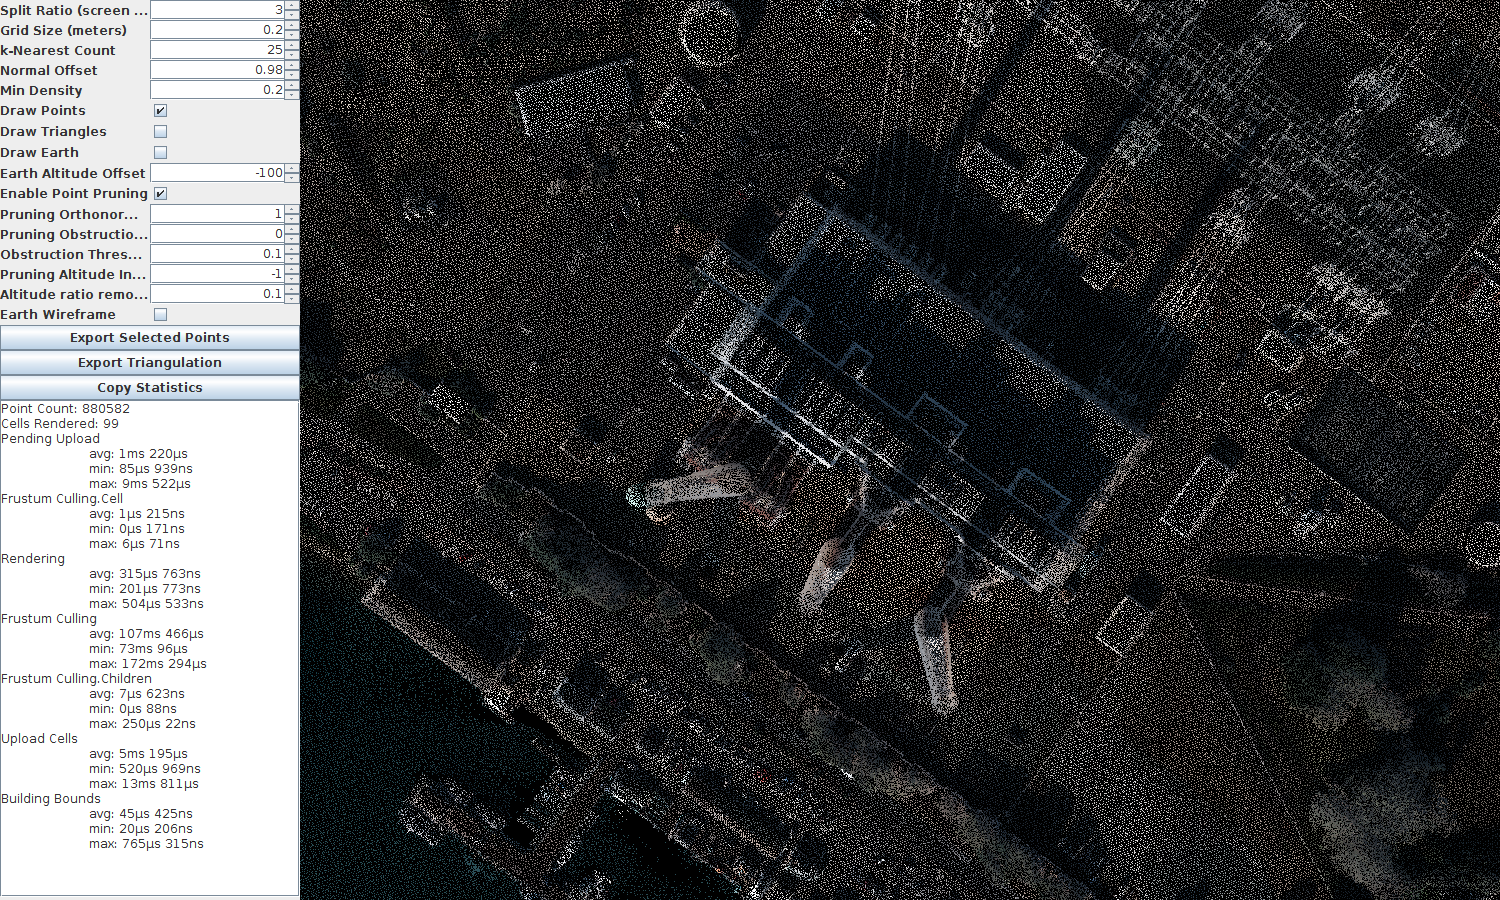
\includegraphics[width=6.0in]{images/rendering3.png}
  \caption{Rendering Statistics Sample Image (depth = 3.0)}
  \label{fig:rendering3}
\end{center}
\end{figure}

%table 7
\begin{table}[htp]
\caption{Rendering Statistics (depth = 6.0)}
\resizebox{\textwidth}{!}{%
  \begin{tabular}{llllll}
    \toprule
      Cell Type & Point Count & Cell Count & Culling & Rendering & Building Bounds \\
    \midrule
      Icosatree (100x100) & 2391155 & 494 & 138 ms & 910 $\mu$s & 310 $\mu$s \\
      Icosatree (150x100) & 4368414 & 494 & 92 ms & 630 $\mu$s & 140 $\mu$s \\
      Icosatree (200x100) & 6239669 & 493 & 110 ms & 502 $\mu$s & 87 $\mu$s \\
      Octree (AABB) & 1915896 & 223 & 126 ms & 312 $\mu$s & 46 $\mu$s \\
    \bottomrule 
  \end{tabular}}
\label{table:renderStats6}
\end{table}

\begin{figure}[htp]
\begin{center}
  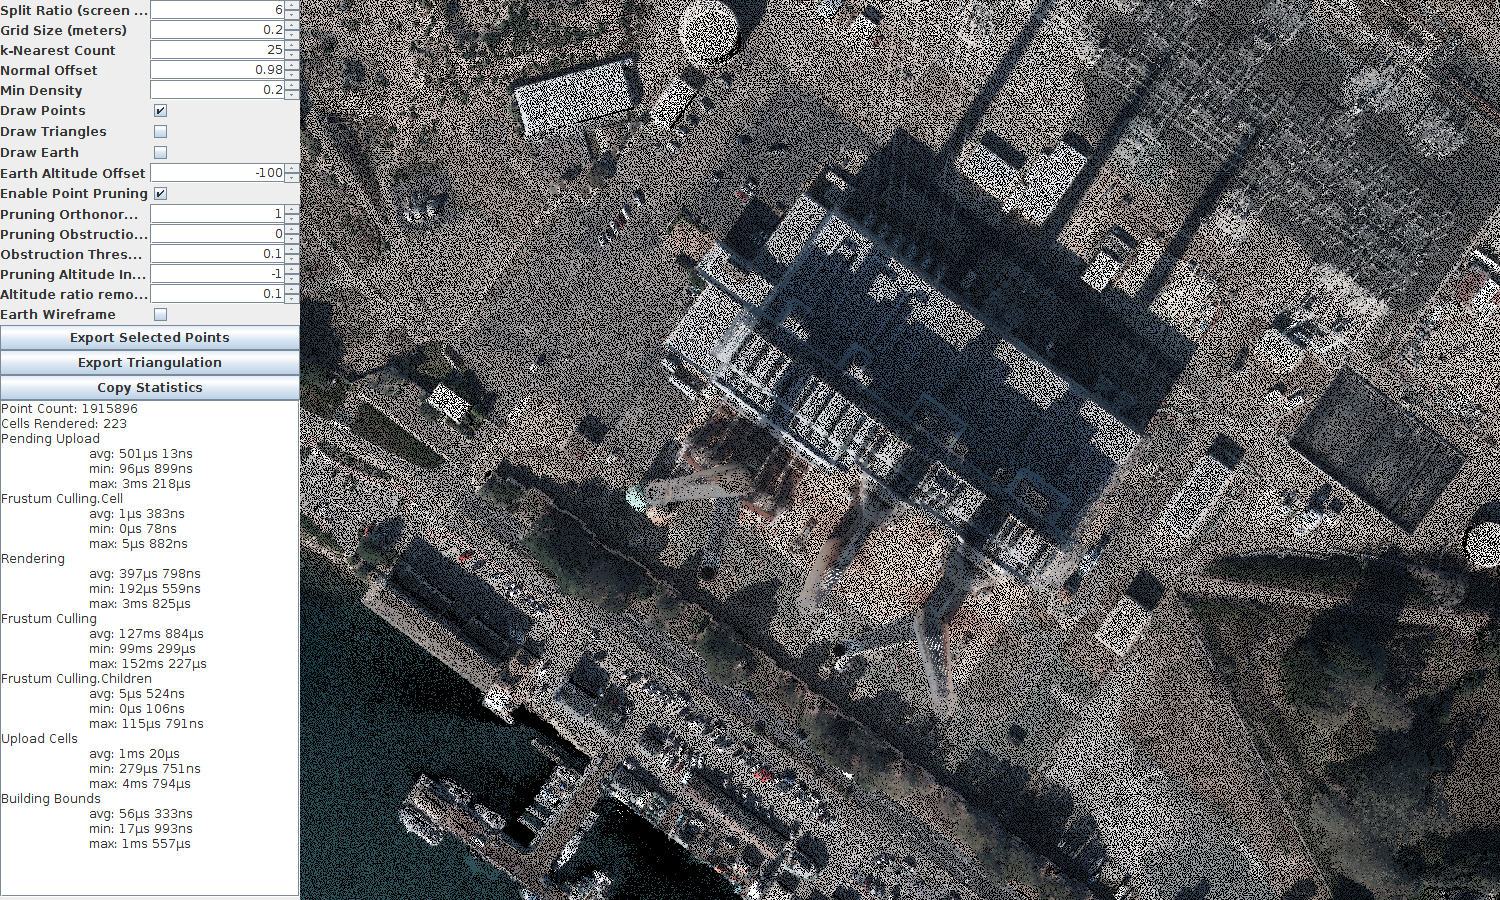
\includegraphics[width=6.0in]{images/rendering6.png}
  \caption{Rendering Statistics Sample Image (depth = 6.0)}
  \label{fig:rendering6}
\end{center}
\end{figure}

























